\paragraph{DVC by Iterative}
Another solution, suitable for ML learning may be DVC \cite{DVC}. DVC achieves
faster data retrieval by its data staying in place. In addition, DVC also uses a
caching layer (Figure \ref{fig:dvc-architecure}), which allows faster data
retrieval for multiple members of team \cite{comparison}. DVC supports both
structured and unstructed data. It however does not support RDBMS. Since it
caters to data scientists, it offers several features which greatly lead to
higher reproducibility, such as defining data pipelines
\cite{dvc-define-pipelines}, visualisation of pipelines
\cite{dvc-run-pipelines}, experiment tracking \cite{dvc-compare-experiments} and
hydra compatibility \cite{dvc-hydra}. It also does not scale as well, mostly due
to the same reasons as git.

\begin{figure}[H]
    \centering
    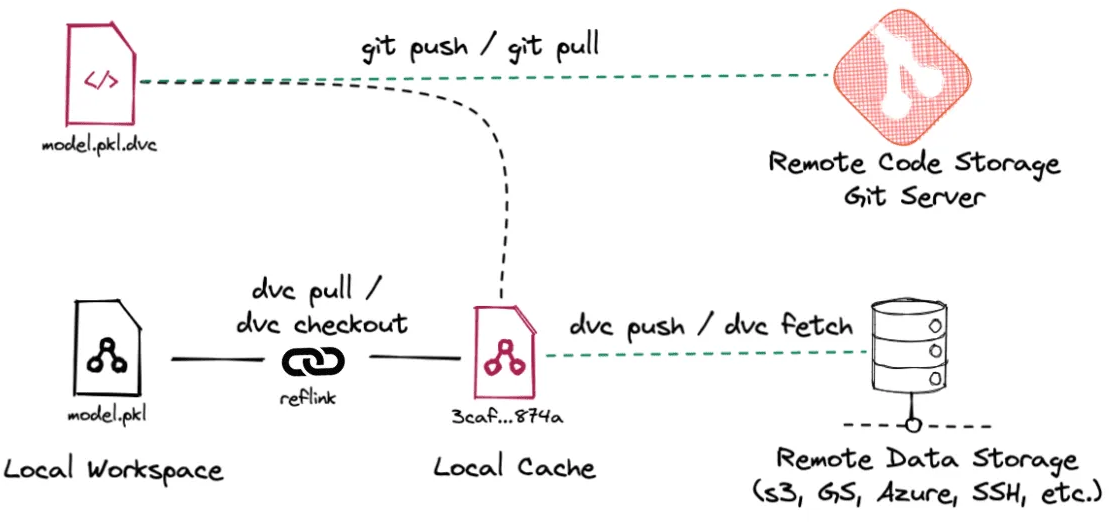
\includegraphics[width=0.8\textwidth]{fig/dvc-arch.png}
    \caption{Software architecture of DVC \cite{comparison}}
    \label{fig:dvc-architecture}
\end{figure}

\begin{comment}
Iterative offers DVC \cite{DVC}, which allows users to save and track model data
and models. Data and models are captured using git commits and can be stored
both locally or in cloud. DVC works by creating metafiles, that describe data to
be tracked. metafiles are put in Git instead of large files.
\end{comment}